\documentclass[12pt]{article}

\usepackage[utf8]{inputenc}
\usepackage{latexsym,amsfonts,amssymb,amsthm,amsmath}
\usepackage{tikz}
\usepackage{stanli}
\usetikzlibrary{shapes,calc,through,3d,patterns}
\usetikzlibrary{arrows.meta,decorations.pathreplacing,angles,quotes}
\usepackage{multicol}
\usepackage{geometry}
\usepackage{mathtools}
\usepackage{siunitx}
\usepackage{booktabs}
\usepackage{tabularx}


\setlength{\parindent}{0in}
\setlength{\oddsidemargin}{-0.25in}
\setlength{\textwidth}{7in}
\setlength{\textheight}{9.3in}
\setlength{\topmargin}{-1in}
\setlength{\headheight}{18pt}

\newcommand\blfootnote[1]{%
    \begingroup
    \renewcommand\thefootnote{}\footnote{#1}%
    \addtocounter{footnote}{-1}%
    \endgroup
}

\definecolor{darkred}{rgb}{0.6,0,0}

\newcommand{\bolddelta}{\boldsymbol\delta}
\newcommand{\boldxi}{\boldsymbol\xi}

\newcolumntype{M}[1]{>{\centering\arraybackslash}m{#1}}


\begin{document}

\noindent
\begin{minipage}[b]{320pt}
	\begin{flushleft}
		\textbf{ME-473}\\
		\textbf{Dynamic finite element analysis of structures}\\
		Stefano Burzio\\
		2024-2025
	\end{flushleft}
\end{minipage}
\hfill
\begin{minipage}[b]{80pt}
	\begin{flushright}
		
\includegraphics[scale=0.6]{../images/epfl-logo.pdf}
		\vspace{0.3cm}
	\end{flushright}
\end{minipage}

\vspace{0.5cm}
\hrulefill
\vspace{0.5cm}

\hspace*{\fill}\textbf{\Large Final exam}\hspace*{\fill}

\hrulefill

\noindent
\begin{tabularx}{\textwidth}{p{6cm}r}
	\hline
	 &                                                                                                                                                             \\
	\multicolumn{2}{l}{First name : .............................................................................................................................} \\[15pt]
	\multicolumn{2}{l}{Last name : ..............................................................................................................................} \\
	[15pt]
	\multicolumn{2}{l}{SCIPER : .................................................................................................................................} \\
	\hline
\end{tabularx}


\noindent
\begin{center}
	\fbox{
		\parbox{160mm}{\centering
			\mbox{}
			\vspace{2mm}
			\begin{itemize}
				\setlength\itemsep{-1mm}
				\item Duration: 150 minutes.
				\item The exam is open book.
				\item Place your student ID card on the table.
				\item The use of a calculator is allowed.
				\item The use of any other electronic device is strictly prohibited during the exam.
			\end{itemize}
			\vspace{-1mm}
			\mbox{}

			\setlength{\tabcolsep}{18pt}
			\renewcommand{\arraystretch}{2}
			\begin{center}
				\begin{tabular}{@{} |l|M{6cm}| @{}}
					\hline
					Problem 1                     & \hspace{3cm}/ 25 points \\[10pt] \hline
					Problem 2                     & \hspace{3cm}/ 25 points \\[10pt] \hline
					\textbf{\emph{Sum of points}} & \hspace{3cm}/ 50 points \\[10pt] \hline
					\textbf{\emph{Final grade}}   &                         \\[10pt] \hline
				\end{tabular}
			\end{center}
		}
		\newline

	}



\end{center}




\newpage




\subsection*{Problem 1 {\small (25 points)}}
Consider the two-dimensional truss structure illustrated in the figure below. The structure consists of four linear elastic truss elements. Elements 1, 2, and 4 share identical constant mechanical and geometric properties, each having a modulus of elasticity $E$, a cross-sectional area $A$, and a mass density $\rho$. In contrast, the diagonal element (element 3) possesses enhanced stiffness and size, characterized by a modulus of elasticity of $25E$, a cross-sectional area of $5A$, while maintaining the same mass density $\rho$. Note that the support at node 2 permits displacements in the horizontal direction.

\begin{center}
	\begin{tikzpicture}[]
		% Nodes
		\coordinate (1) at (0,0);
		\coordinate (2) at (3,0);
		\coordinate (3) at (3,4);
		\coordinate (4) at (0,4);
		%Supports 
		\point{a}{0}{0};
		\point{b}{0}{4};
		\point{c}{3}{0};
		\point{d}{3}{4};
		\support{1}{a}[-90];
		\support{1}{b}[-90];
		\support{2}{c};
		%\support{2}{d}[90];
		% Members
		\draw[ultra thick] (1) -- (2);
		\draw[ultra thick] (3) -- (1);
		\draw[ultra thick] (2) -- (3);
		\draw[ultra thick] (3) -- (4);
		\draw[thick] (1.5,0.3) circle(0.2cm);
		\node at (1.5,0.3) {1};
		\draw[thick] (3.3,2) circle(0.2cm);
		\node at (3.3,2) {2};
		\draw[thick] (1.1,2) circle(0.2cm);
		\node at (1.1,2) {3};
		\draw[thick] (1.5,4.3) circle(0.2cm);
		\node at (1.5,4.3) {4};
		% Points
		\node[below=1pt,darkred] at (1) {1};
		\node[above right=1pt,darkred] at (2) {2};
		\node[above right=1pt,darkred] at (3) {3};
		\node[below=1pt,darkred] at (4) {4};
		% Axes
		\draw[-latex,  thin, darkred] (1) -- ++(1,0) node[below] {$x$};
		\draw[-latex,  thin, darkred] (1) -- ++(0,1) node[right] {$y$};
		% Dimensions 
		\draw[ultra thin] (3,0) -- (4,0);
		\draw[ultra thin] (3,4) -- (4,4);
		\draw[ultra thin,latex-latex] (3.8,0) -- (3.8,4) node[midway, right] {$4$ m};
		\draw[ultra thin] (3,4) -- (3,5);
		\draw[ultra thin] (0,4) -- (0,5);
		\draw[ultra thin,latex-latex] (0, 4.8) -- (3,4.8) node[midway, above] {$3$ m};
		% Pins
		\draw[thick,fill=white] (3) circle (3pt);
		\draw[thick,fill=white] (2) circle (3pt);
		\draw[thick,fill=white] (1) circle (3pt);
		\draw[thick,fill=white] (4) circle (3pt);
		% Wheels 
		\draw [thick] (2.70,-0.55) circle [radius=0.05];
		\draw [thick] (3.00,-0.55) circle [radius=0.05];
		\draw [thick] (3.30,-0.55) circle [radius=0.05];
		%\draw [thick] (3.55,4.3) circle [radius=0.05];
		%\draw [thick] (3.55,4) circle [radius=0.05];
		%\draw [thick] (3.55,3.7) circle [radius=0.05];
	\end{tikzpicture}
\end{center}

\begin{enumerate}
	\item[(a)] (2 points) Based on the finite element discretization, determine the total number of degrees of freedom in the structure. Clearly distinguish between those degrees of freedom that are constrained by the boundary conditions and those that are unconstrained.
	\item[(b)] (6 points) Compute the elementary stiffness matrices and assemble them to obtain the global stiffness matrix. Verify that the reduced stiffness matrix corresponding to the unconstrained degrees of freedom of the structure is
	      $$\mathbf K_{red}=EA\begin{bmatrix}
			      1/3 & 0    & 0    \\
			      0   & 28/3 & 12   \\
			      0   & 12   & 65/4 \\
		      \end{bmatrix}$$
	\item[(c)] (6 points) Given the reduced consistent mass matrix
	      $$\mathbf{M}_{red}=\rho A \begin{bmatrix}
			      1 & 0 & 0 \\
			      0 & 4 & 4 \\
			      0 & 4 & 6 \\
		      \end{bmatrix},$$
	      formulate the generalized eigenvalue problem. Compute the three lowest natural frequencies, and the fundamental mode shape of the structure. Can you provide a physical interpretation of the fundamental mode shape? To simplify the numerical computation, assume normalized parameters \( E = A = \rho = 1 \).
	\item[(d)] (2 points) You are asked to design a structure with the highest possible fundamental frequency. Based on your knowledge of material and geometric properties, explain how you would choose the parameters: $E$, $A$, and $\rho$.
	\item[(e)] (6 points)  For this point, node 3 is constrained to vertical displacement only and subjected to a time-harmonic vertical load of magnitude
	      \[
		      f(t) = a \sin(\bar\omega t)
	      \]
	      where \( a \) and \( \bar\omega \) are given constants. Assuming the structure is initially at rest with zero initial velocity, compute the transient response \( \mathbf{q}_r(t) \) for \( t\in]0,T[ \) and identify the value(s) of $\bar\omega$ that will cause the structure to resonate. To simplify the numerical computation, assume normalized parameters: \( E = A = \rho = 1 \).
	\item[(f)] (3 points) By modifying/removing at most two supports of the given planar truss structure, and/or by removing at most one truss element, provide a sketch of a configuration that has exactly one rigid body mode. Justify briefly your answer.
\end{enumerate}


\subsection*{Problem 2 {\small (25 points)}}
A single tooth of a thin spur gear is modelled in plane stress by the trapezoidal domain \( \Omega \subset \mathbb{R}^2 \) shown below. The tooth is made of an isotropic, homogeneous steel with Young’s modulus \(E\), Poisson ratio \( \nu \) and mass density $\rho$. The tooth is loaded by a uniform tangential traction of magnitude \(q \) applied along the top face \( \overline{CD} \). Along \( \overline{AB} \) (the wheel rim) the displacements are
fully constrained.
\begin{center}
	\begin{tikzpicture}[scale=0.09]
		% Coordinates
		\coordinate (A) at (0,0);
		\coordinate (B) at (40,0);
		\coordinate (C) at (35,30);
		\coordinate (D) at (5,30);
		\coordinate (E) at (20,0);
		% Supports along AD 
		\draw[white, pattern=north east lines,pattern color=black] (A)--
		(B) -- (40,-6) -- (0,-6) -- cycle;
		% Domain
		\filldraw[fill=gray!30,draw=black,thick] (A)--(B)--(C)--(D)--cycle;
		\node at (20,15) {\small $\Omega$};
		% Node dots & labels
		\node[left] at (A) {\small $A$};
		\node[right] at (B) {\small $B$};
		\node[right] at (C) {\small $C$};
		\node[left] at (D) {\small $D$};
		% Traction arrows on CD
		\foreach \x in {30,25,20,15,10,5}{
				\draw[-latex,thick] (\x,30.9)--++(4,0);
			}
		\node[above] at (20,31) {$q$};
		% Axes
		\draw[-latex,thin] (A)--++(10,0) node[above]{$x$};
		\draw[-latex,thin] (A)--++(0,10) node[above]{$y$};
	\end{tikzpicture}
\end{center}

\begin{itemize}
	\item[(a)] (6 points) Write the strong form of the two-dimensional plane-stress problem and derive the corresponding weak form: find \( \mathbf{u}\in\mathcal{U} \) such that
	      \[
		      \int_{\Omega} (\nabla \bolddelta\mathbf  u )^T
		      \mathbf{C}\,\nabla \mathbf{u}\;d\Omega +  \int_{\Omega}
		      \rho(\bolddelta\mathbf  u )^T
		      \ddot{\mathbf{u}}\;d\Omega
		      = \int_{\Gamma_\sigma} (\bolddelta\mathbf  u)^T\mathbf{t}\,d\Gamma
		      \qquad \forall\, \bolddelta\mathbf  u \in\mathcal{V}.
	      \]
	      Specify the functional spaces \( \mathcal{U}\) and \(\mathcal{V} \), the boundary $\Gamma_\sigma$, the matrix $\mathbf C$, the force vector $\mathbf t$, and the operator $\nabla$.

	\item[(b)] (3 points) The domain is discretised with three triangular bilinear finite elements, as indicated in the mesh below.
	      \begin{center}
		      \begin{tikzpicture}[scale=0.09]
			      % Coordinates
			      \coordinate (A) at (0,0);
			      \coordinate (B) at (40,0);
			      \coordinate (C) at (35,30);
			      \coordinate (D) at (5,30);
			      \coordinate (E) at (20,0);
			      % Domain
			      \filldraw[fill=gray!30,draw=black,thick] (A)--(B)--(C)--(D)--cycle;
			      \node at (19,15) {\small ${}^2\Omega$};
			      \node at (7,10) {\small ${}^1\Omega$};
			      \node at (31,10) {\small ${}^3\Omega$};

			      % Node dots & labels
			      \fill[black] (A) circle (1cm);
			      \fill[black] (B) circle (1cm);
			      \fill[black] (C) circle (1cm);
			      \fill[black] (D) circle (1cm);
			      \fill[black] (E) circle (1cm);
			      \node[below] at (A) {\small $1$};
			      \node[below] at (B) {\small $2$};
			      \node[right] at (C) {\small $3$};
			      \node[left] at (D) {\small $4$};
			      \node[below] at (E) {\small $5$};
			      % Axes
			      \draw[-latex,thin] (A)--++(10,0) node[above]{$x$};
			      \draw[-latex,thin] (A)--++(0,10) node[above]{$y$};
			      % Mesh (3 CST elements)
			      \draw[thick] (A)--(E)--(B);
			      \draw[thick] (E)--(C);
			      \draw[thick] (E)--(D);
		      \end{tikzpicture}
	      \end{center}
	      Determine the transformation ${}^1T : {}^a\Omega \to {}^1\Omega$ that maps the reference triangle ${}^a\Omega$ to the physical triangular element ${}^1\Omega$. Compute the components of the Jacobian matrix ${}^1\mathbf{J}$ associated with the transformation, and evaluate its determinant ${}^1{j}$. The nodes coordinates are:
	      \[
		      \begin{array}{c|cc}
			      \text{Node} & x\;[\text{mm}] & y\;[\text{mm}] \\\hline
			      1           & 0              & 0              \\
			      2           & 40             & 0              \\
			      3           & 35             & 30             \\
			      4           & 5              & 30             \\
			      5           & 20             & 0
		      \end{array}
	      \]

	\item[(c)] (2 points) For the given discretization, specify the dimensions of the following matrices:

	      \begin{itemize}
		      \item[(i)] The elementary stiffness matrices ${}^e \mathbf{K}$;
		      \item[(ii)] The assembled global stiffness matrix $\mathbf{K}$;
		      \item[(iii)]  The reduced stiffness matrix $\mathbf{K}_{red}$, obtained after imposing the boundary conditions.
	      \end{itemize}

	\item[(d)] (4 points) For the given discretization, write the expression of the elementary consistent mass matrix ${}^e\mathbf{M}$ in terms of the shape functions ${}^eh_i$. Then, compute the entries ${}^1\mathbf M_{12}$ and ${}^1\mathbf M_{13}$.

	\item[(e)] (4 points) To enhance the accuracy of the approximated fundamental frequency obtained from the generalized eigenvalue problem, consider the two alternatives mesh listed below. Rank these mesh options in order of increasing accuracy with respect to the fundamental frequency approximation, and justify your answer.
	      \begin{multicols}{2}
		      \begin{itemize}
			      \item[(i)] 12 bilinear triangular elements;
			            \begin{center}
				            \begin{tikzpicture}[scale=0.09]
					            % Coordinates
					            \coordinate (A) at (0,0);
					            \coordinate (B) at (40,0);
					            \coordinate (C) at (35,30);
					            \coordinate (D) at (5,30);
					            \coordinate (E) at (20,0);
					            \coordinate (F) at (2.5,15);
					            \coordinate (G) at (12.5,15);
					            \coordinate (H) at (20,30);
					            \coordinate (I) at (27.5,15);
					            \coordinate (J) at (37.5,15);
					            \coordinate (M) at (10, 0);
					            \coordinate (N) at (30,0);
					            % Domain
					            \filldraw[fill=gray!30,draw=black,thick] (A)--(B)--(C)--(D)--cycle;
					            % Node dots & labels
					            \foreach \P in {A, B, C, D, E, F, G, I, J, M, N, H} {
							            \fill[black] (\P) circle (1cm);
						            }
					            % Mesh (3 CST elements)
					            \draw[thick] (A)--(E)--(B);
					            \draw[thick] (E)--(C);
					            \draw[thick] (E)--(D);
					            \draw[thick] (F)--(G)--(M) -- cycle;
					            \draw[thick] (G)--(H) -- (I)  -- cycle;
					            \draw[thick] (I)--(N)--(J) -- cycle;

				            \end{tikzpicture}
			            \end{center}
			      \item[(ii)] 3 biquadratic triangular elements;
			            \begin{center}
				            \begin{tikzpicture}[scale=0.09]
					            % Coordinates
					            \coordinate (A) at (0,0);
					            \coordinate (B) at (40,0);
					            \coordinate (C) at (35,30);
					            \coordinate (D) at (5,30);
					            \coordinate (E) at (20,0);
					            \coordinate (F) at (2.5,15);
					            \coordinate (G) at (12.5,15);
					            \coordinate (H) at (20,30);
					            \coordinate (I) at (27.5,15);
					            \coordinate (J) at (37.5,15);
					            \coordinate (M) at (10, 0);
					            \coordinate (N) at (30,0);
					            % Domain
					            \filldraw[fill=gray!30,draw=black,thick] (A)--(B)--(C)--(D)--cycle;
					            % Node dots & labels
					            \foreach \P in {A, B, C, D, E, F, G, I, J, M, N, H} {
							            \fill[black] (\P) circle (1cm);
						            }
					            % Mesh (3 CST elements)
					            \draw[thick] (A)--(E)--(B);
					            \draw[thick] (E)--(C);
					            \draw[thick] (E)--(D);
				            \end{tikzpicture}
			            \end{center}

		      \end{itemize}
	      \end{multicols}

	\item[(f)] (4 points) For the discretization given below, consisting of a single bicubic quadrilateral element, determine the minimum number of Gauss points required in the Gauss quadrature to evaluate exactly the mass matrix ${}^e\mathbf{M}$, and provide a justification.  Repeat the analysis for the element stiffness matrix ${}^e\mathbf{K}$.
	      \begin{center}
		      \begin{tikzpicture}[scale=0.09]
			      % Coordinates
			      \coordinate (A) at (0,0);
			      \coordinate (B) at (40,0);
			      \coordinate (C) at (35,30);
			      \coordinate (D) at (5,30);
			      \coordinate (F) at (5/3,30/3);
			      \coordinate (G) at (10/3,60/3);
			      \coordinate (H) at (35+10/3,30/3);
			      \coordinate (I) at (35+5/3,60/3);
			      \coordinate (J) at (15,30);
			      \coordinate (K) at (25,30);
			      \coordinate (M) at (13.3, 0);
			      \coordinate (N) at (26.3,0);
			      \coordinate (P) at (5/3+110/9,30/3);
			      \coordinate (Q) at (5/3+220/9,30/3);
			      \coordinate (R) at (10/3+100/9,60/3);
			      \coordinate (S) at (10/3+200/9,60/3);
			      % Domain
			      \filldraw[fill=gray!30,draw=black,thick] (A)--(B)--(C)--(D)--cycle;
			      % Node dots & labels
			      \foreach \P in {A, B, C, D,F, G, I, J, M, N, H, K, P, Q, R, S} {
					      \fill[black] (\P) circle (1cm);
				      }
		      \end{tikzpicture}
	      \end{center}
	\item[(g)] (2 points) The Newmark time integration method with parameters $\beta = \frac{1}{4}$ and $\gamma = \frac{1}{2}$ is widely employed in structural dynamics. Determine whether this scheme is explicit or implicit, and provide a brief justification. Explain why it is referred to as the average acceleration method.
\end{itemize}


\end{document}